%-------------------------------------------------------------------------%
\section{Possible decay channels of the top squarks} 
\label{sec:stopDecay}
Just as the SM particles and their decays are determined by symmetries, couplings, and masses of the particles involved, the decay of stops is also determined by parameters in the MSSM. The mass of stops would determine the favorable decay modes. The top squarks have two gauge eigenstates that mix strongly due to the large top quark mass. This results in mass eigenstates of two top squarks, the lighter of which is possibly lighter than other supersymmetric particles other than the neutralinos \cite{thomson2013modern, boehm2000decays}. The important assumption made in these decays is that the stops are heavier than the neutralino ($m_{\Tilde{t}} > m_{\Tilde{\chi}_1^0} $) so that the neutralinos is the LSP. \\

A heavy enough stop with a mass heavier than the sum of the top quark mass and neutralino mass ($m_{\Tilde{t}} > m_t+m_{\Tilde{\chi}_1^0}$) would undergo a two-body decay into a quark with neutralinos: $\Tilde{t}\rightarrow q\Tilde{\chi}_1^0$. In reference \cite{boehm2000decays}, the charm quark pair produced with the neutralino is considered the dominant process from a low-mass top squark and high-mass neutralino, but in this project we approach the simplified model that is the other possible decay in the MSSM; top squarks to top quark-neutralino pair $\Tilde{t}\rightarrow t\Tilde{\chi}_1^0$. A lighter stop that is heavier than the sum of the bottom quark mass, W-boson mass and neutralino mass ($m_{\Tilde{t}} > m_b + m_W + m_{\Tilde{\chi}_1^0}$), but the mass difference between the stops and neutralinos ($\Delta m = m_{\Tilde{t}} - m_{\Tilde{\chi}_1^0} $) is lighter than the top quark ($\Delta m < m_t$) allows a three-body decay with virtual W bosons in the process $\Tilde{t}\rightarrow b W \Tilde{\chi}_1^0$. Further decays are apparent when supersymmetric particles other than $\Tilde{\chi}_1^0 $ are lighter than the stop, for example, the charginos $\Tilde{\chi}_1^{\pm}$. If $\Tilde{\chi}_1^{\pm}$ is lighter than the stops, the decay results in a bottom quark-chargino pair: $\Tilde{t}\rightarrow b\Tilde{\chi}_1^+$ \cite{boehm2000decays}. \\

%would imply a three-body decay  Four-body decays into a combination of bottom quarks, neutralinos and SM fermions, may also be possible: $\Tilde{t}\rightarrow b\Tilde{\chi}_1^0 f \Bar{f}'$ \cite{boehm2000decays}. However, the four-body decay is only relevant when the two- and three-body decays are kinematically forbidden. This would also allow a flavor-suppressed decay to a charm quark: $\Tilde{t}\rightarrow c\Tilde{\chi}_1^0$ \cite{aad2014search}. \\

A diagram from \cite{aad2014search} is shown in Figure \ref{fig:decayMode}, reflecting the statements above under the assumption that $ \Tilde{\chi}_1^0 $ and $\Tilde{t}$\footnote{The SM quarks have a left- and right-handed component in which they are a doublet and a singlet respectively. The MSSM counterpart also has left- and right-handed components that mix to form two distinct squarks, hence the notation $\Tilde{t}_1$ for the lighter stops in Figure \ref{fig:decayMode}.} are the lightest and next-to-lightest particles in the MSSM. For this project, we stick to a simplified model with final states that include one charged lepton, some missing energy and some hadronic jets as shown in Figure \ref{fig:stopDecay}. The
desired background events are the process given by Equation (\ref{eq:background}) and the desired signal events are given by Equation (\ref{eq:signal}), in which the $b$-quarks originates from the decay $t\Bar{t} \rightarrow bW^+ \Bar{b}W^-$ and are detected as $b$-jets. \\

\begin{equation}
 pp \rightarrow t \Bar{t} \rightarrow b\Bar{b}jjl\cancel{\it{E}}_{T},
 \label{eq:background}
\end{equation}
\begin{equation}
  pp \rightarrow \Tilde{t}\Tilde{t^*} \rightarrow t \Bar{t} \Tilde{\chi^0_1}\Tilde{\chi^0_1} \rightarrow b\Bar{b}jjl\cancel{\it{E}}_{T},
  \label{eq:signal}
\end{equation}

%The doublet allows mixing with other quarks (e.g. tops with the bottom) thus making them more complicated and potentially heavier.
\begin{figure}[htbp]
    \centering
    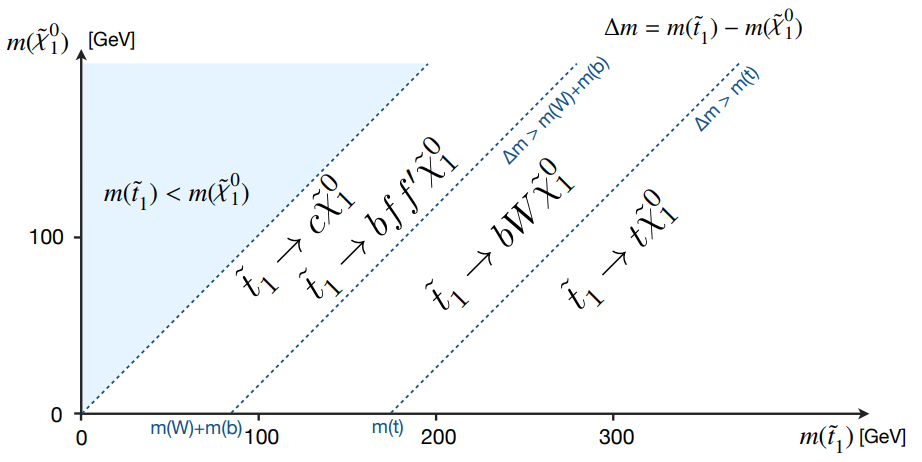
\includegraphics[width=0.75\linewidth]{decaymodes.png}
    \caption{Possible decay modes for stops within the mass-parameter space of $\Tilde{t}_1 $ and $ \Tilde{\chi}_1^0 $ \cite{aad2014search}. The blue filled region is kinematically forbidden due to the neutralino mass being heavier than the stop mass. As the mass of stops get heavier, the allowed decays differ, favoring on-shell decays over off-shell decays.}
    \label{fig:decayMode}
\end{figure}


\begin{figure}[htbp]
    \centering
    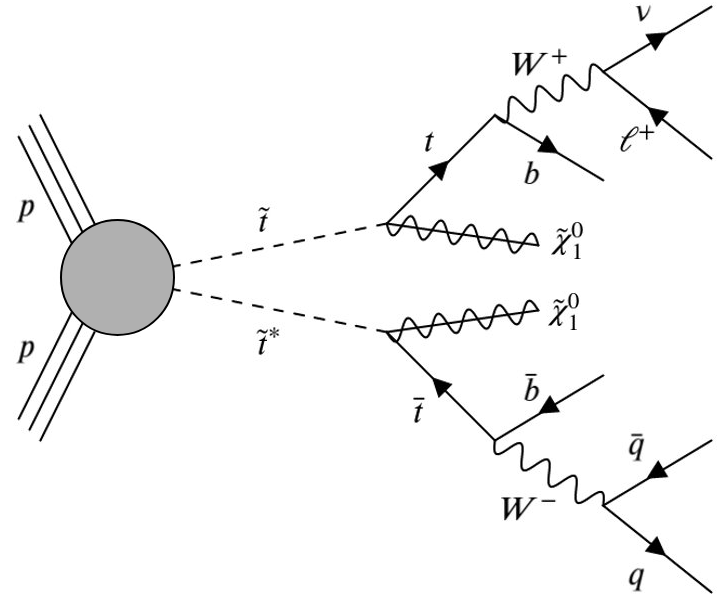
\includegraphics[width=0.5\linewidth]{stop_decay2.png}
    \caption{An example decay of the signal of interest $\Tilde{t}\Tilde{t}^* \rightarrow t\bar{t}\Tilde{\chi}_1^0\Tilde{\chi}_1^0 $ with a final state of one charged lepton-neutrino pair, and hadronic jets originating from the quark-antiquark pairs and bottom quarks.}
    \label{fig:stopDecay}
\end{figure}


%-------------------------------------------------------------------------%
%\section{Mass of the top squark}
%\label{sec:stopMass}
%The mass eigenstates for the top squarks are given by the equation

%\begin{align}
%    \begin{pmatrix} \Tilde{t}_1 \\ \Tilde{t}_2 \end{pmatrix} = 
%    \begin{pmatrix} \cos\theta_\Tilde{t} & -\sin\theta^*_\Tilde{t} \\ \sin\theta_\Tilde{t} & \cos\theta^*__\Tilde{t} \end{pmatrix}
%    \begin{pmatrix} \Tilde{t}_L \\ \Tilde{t}_R \end{pmatrix}
%    \label{eq:stopMass}
%\end{align}
%where $ \theta_\Tilde{t} $ is the stop mixing angle in the range $ 0 \leq {\theta_\Tilde{t}} \leq \pi $ satisfying $ |\cos\theta_{\Tilde{t}}|^2 + |\sin\theta_{\Tilde{t}}|^2 = 1 $ \cite{martin1997supersymmetry}. \\

%The mass splitting of the two stops $ \tilde{t}_1 $ and $ \tilde{t}_2 $ arise from the squared-mass matrix for stops, where the off-diagonal elements involves a large top-quark Yukawa coupling ($y_t$ term) that induces such a phenomena \cite{kraml2016scalar}. Diagonalizing gives the $\Tilde{t}_L$ and $\Tilde{t}_R$ components on the right-hand side of Equation (\ref{eq:stopMass}). One possible model in the MSSM predicts that $\Tilde{t}_1$ is the lightest of all squarks predominantly theorized to be $\Tilde{t}_R$ which is the right-handed stops \cite{martin1997supersymmetry}. Although there has been no success in the direct detection of the particle, experimental efforts have been made to set constraints on its mass \cite{kraml2016scalar, aad2014search, abdughani2018probing, sirunyan2018search, yoshihara2017search}.

%-------------------------------------------------------------------------%
\section{Mass parameters for the top squarks and neutralinos}
Experiments at the Large Hadron Collider have set limits on the stop mass and neutralino mass since the operation began in 2008. Several searches have been made for new particles and their properties with statistical techniques to establish limits, and make a discovery in a fortunate scenario such as the Higgs boson. A frequentist approach, in short, is the main statistical technique taken where a numerical analysis is based on a probability-based hypothesis test.

%-------------------------------------------------------------------------%
\subsection{Frequentist statistics - setting limits in searches}
\label{sec:freqStat}
%A likelihood function provides us with the probability distribution function evaluated for the observed data, in which the extended likelihood function to account for the Poisson distribution of the number of events $N$ is given by
%\begin{equation}
%    L(\vec{x}_1,...,\vec{x}_n; \vec{\theta}) 
%    = \frac{e^{-\mu_n(\vec{\theta})}\mu_n(\vec{\theta})}{n!}\prod^n_{i=1} f(\vec{x}_i;\vec{\theta})
%    \label{eq:genLikelihood}
%\end{equation}
%where $\vec{x}_i$ is an individual observation in a set of $i=1,...,n$ random variables amongst $N$ number of uncorrelated events, $\mu_n(\vec{\theta})$ is the expected number of events dependant on some nuisance parameter $\vec{\theta}$, a parameter in which unknown parameters coupled to the parameter of interest from detector response is accounted for \cite{lista2017statistical}.
The hypothesis test most commonly used in collider experiments is a background-only (null) hypothesis $H_0$  $(b)$. The alternate hypothesis  $H_1$ then includes both signal and background events $(s+b)$. In the absence of systematic uncertainties, one can construct the likelihood ratio evaluated with likelihoods\footnote{Collider experiments are considered a form of counting experiment. The observed events assume a Poisson distribution with a mean of $\mu_s+\mu_b$ where $\mu_{s(b)}$ is the estimated number of signal(background) \cite{lista2017statistical, adam-bourdarios_learning_2014}, hence the likelihood is $P(n|\mu_s,\mu_b) = \frac{(\mu_s+\mu_b)^n}{n!}e^{-(\mu_s+\mu_b)}$} $L(\mu)$ \cite{LHCstats}; $H_0 \rightarrow L_{s+b}$ and $H_1 \rightarrow L_b$ given by
\begin{equation}
    \lambda(\mu) = \frac{L_{s+b}}{L_b}
    %(\mu, \hat{\hat{\theta}}), (\hat{\mu},\hat{\theta})
    \label{eq:genLR}
\end{equation}
%for some maximum-likelihood estimators\footnote{The maximum likelihood estimators provide the parameter values that maximize the search for a particular observation within the set.} $\hat{\mu}$ and $\hat{\theta}$, and $\hat{\hat{\theta}}$ being the conditional maximum-likelihood estimator \cite{cowan2011asymptotic}. \footnote{The signal discovery test statistic is $q_0$ where it holds the value $-2 \ln \lambda (0)$ for $\hat{\mu}=0$ and zero otherwise.}
where $\lambda$ is in the range $0 \leq \lambda \leq 1$. Equation (\ref{eq:genLR}) is then used in a test statistic $q_\mu$ defined as
\begin{equation}
    q_\mu = \left\{
        \begin{array}{ll}
            -2\ln \lambda(\mu) & \quad \hat{\mu} \leq \mu \\
            0 & \quad \hat{\mu} \geq \mu
        \end{array}
    \right.
\end{equation}
for some signature $\mu$ (0 for $H_0$ and 1 for $H_1$) and its effective estimator $\hat{\mu}$ that maximizes the likelihood. For a hypothesis assuming $\mu$, the incompatibility of the hypothesis with the data results in a large $q_\mu$. This is further quantified with a \textit{p-value} given by the probability distribution function (pdf) of the test statistic $q_\mu$, $f(q_\mu|\mu)$, integrated over the tail of its distribution with some observation \cite{cowan2011asymptotic}, expressed as \\
\begin{equation}
    p_\mu = \int\limits^\infty_{q_{\mu,obs}} f(q_\mu|\mu) dq_\mu
    \label{eq:p-value}
\end{equation}

In placing limits, physicists use the confidence level $CL_\mu$ that inverts the integral in Equation (\ref{eq:p-value}) to give
\begin{equation}
    CL_\mu = \int\limits_{-\infty}^{q_{\mu,obs}} f(q_\mu|\mu) dq_\mu
    \label{eq:CLmu}
\end{equation}
where $\mu$ is testing for the background $b$ or the signal plus background $s+b$ case, instead of background versus signal. The pdf of both $b$ and $s+b$ overlap when the number of expected signal is extremely low, supporting neither hypothesis.
The signal confidence level $CL_s$ prevents accidental exclusions from the incorrect inference of p-values to such cases, as $CL_s$ lacks frequentist coverage in parameter regions where experiments are insensitive to the expected signal \cite{LHCstats}. The $CL_s$ is given as a ratio of the p-values of the two hypotheses:
\begin{equation}
    CL_s = \frac{CL_{s+b}}{CL_b} \rightarrow \frac{p_{s+b}}{1-p_b}
    \label{eq:CLS}
\end{equation}

%This allows us to compute the significance\footnote{For a discovery to be claimed, particle physicists require a minimum of $Z=5$ that corresponds to $p=2.87\times10^{-7}$ when rejecting the background only hypothesis.} $Z$ and its associated $p$-value with the relationship
%\begin{equation}
%    Z = \Phi^{-1}(1-p) = \sqrt{q_\mu}
%    \label{eq:Z}
%\end{equation}
%The exclusion of the hypothesis $\mu$ is supported when a threshold $p=\alpha$ is applied with a low value e.g. $\alpha=0.05$ for a 95\% confidence level ($Z=1.64$) \cite{cowan2011asymptotic}. \\

%Collider experiments are considered a form of counting experiments, thus the observed events are categorized under a Poisson distribution with a mean of $\mu_s+\mu_b$ where $\mu_{s(b)}$ is the estimated number of signal(background) \cite{lista2017statistical, adam-bourdarios_learning_2014}. This gives us a more simplified version to Equation (\ref{eq:genLikelihood});
%\begin{equation}
%    P(n|\mu_s,\mu_b) = \frac{(\mu_s+\mu_b)^n}{n!}e^{-(\mu_s+\mu_b)}
%    \label{eq:Poisson}
%\end{equation}
%whose likelihood ratio is given by
%\begin{equation}
%    \lambda = \frac{P(n|\mu_s,\mu_b)}{P(n|\hat{\mu_s},\mu_b)}
%    \label{eq:likelihoodRatio}
%\end{equation}
%where $\hat{\mu_s}$ is the maximum likelihood estimator of $\mu_s$. \\


%-------------------------------------------------------------------------%
\subsection{Exclusion limits for the stop and neutralino masses}
The exclusion of masses for new particles is performed through statistical analysis of the results. The exclusion of stop and neutralino masses is visually presented as an exclusion curve in CMS and ATLAS, such as those seen in Figure \ref{fig:limits} \cite{cms2019search} where \textit{inside} the expected limit (in red) and observed limit (in black) have already been excluded. \\

\begin{figure}[htbp]
    \centering
    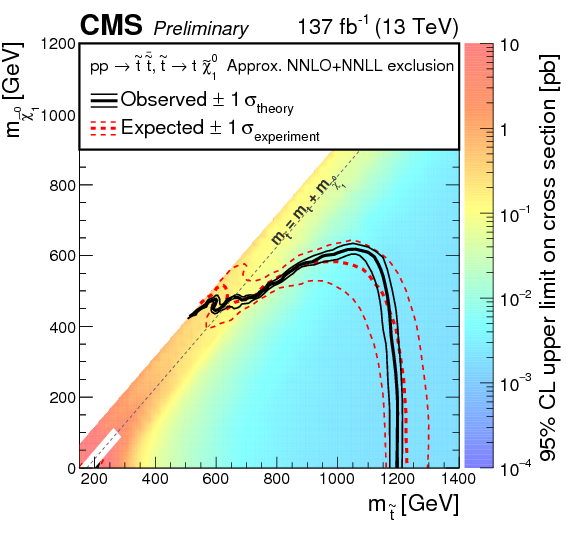
\includegraphics[width=12cm, height= 12cm]{stop_limits.png}
    \caption{The latest cross-section and mass limits for the process $\Tilde{t}\Tilde{t}^* \rightarrow t\bar{t}\Tilde{\chi}_1^0\Tilde{\chi}_1^0 $ set by the CMS experiment \cite{cms2019search}. Inside the black curve are the excluded masses for stops and neutralino, and outside this line remains a  region for allowed masses for these particles, with the stop mass' limit pushed to the TeV scale. According to the colour bar, the further out into to parameter space we travel to, the allowed cross-section is extremely small at the order of $10^{-2}$pb.}
    \label{fig:limits}
\end{figure}

In this particular figure, it is presented that the expected limit to the process $pp \rightarrow \tilde{t}\tilde{t}^* \rightarrow t\tilde{\chi}_1^0$ falls under that of the observed limit when both masses are high i.e. when stop masses are in the order of 1-1.2TeV and neutralino masses in the order of $\sim600$ GeV. It is also shown that the observed limit falls under the expected limit when there is a massive mass difference between the stop and the neutralino i.e. $m_{\tilde{\chi}_1^0}\ll m_{\tilde{t}}$. Furthermore, the upper limit on the cross-section for the simplified model is provided in colour-code, such that  cross-section values above the corresponding colour will be excluded. This suggests that our signal selection efficiency is high when searching in regions with lower
limits. \\

The masses around $ m_{\tilde{t}} \approx 1.2$ TeV are an interesting range of parameters to follow, mainly to observe how the mass difference $\Delta m$ affects the performance of our machine learning classifiers. Intuitively, the large difference implies that the final states are highly energetic compared to the background events, and hence more easily differentiated than when $\Delta m$ is small. In addition, reference \cite{roxlo2018opening} has explored the performance of their neural networks discriminating stop production to top production, albeit in a dilepton final state within the $\tilde{t} \rightarrow t \tilde{\chi}_1^0$ decay. To do a cross-check, their choice of mass parameters are our fourth benchmark point: $m_{\tilde{t}} =750$ GeV and $m_{\tilde{\chi}_1^0} = 1$ GeV, well within the exclusion limit in Figure \ref{fig:limits}. Table \ref{tab:benchmarks} shows a summary of mass parameters chosen to explore. These parameters were chosen particularly to observe the effect of varying $\Delta m$, with a slight change in stop masses to ensure we are choosing masses just outside of the exclusion curve.

\begin{table}[htbp]
    \centering
    \begin{tabular}{c|c|c|c} 
    \toprule
    Benchmark No. & Position & $m_{\Tilde{t}}$ (TeV) & $m_{\Tilde{\chi}_1^0}$ (GeV) \\
    \midrule
    \rowcolor{gray!6} 1 & Outside & $ 1.2 $ & $ 600 $ \\
    2 & Outside & $ 1.225 $ & $ 400 $ \\
    \rowcolor{gray!6} 3 & Outside & $ 1.25 $ & $ 100 $ \\
    4 & Inside & $ 0.75 $ & $ 1 $\\
    \bottomrule
    \end{tabular}
    \caption{Chosen parameters for building classifiers, three of which tracing just outside of the observed exclusion limit in Figure \ref{fig:limits}, and one of which is completely inside the curve, following that of \cite{roxlo2018opening}. In doing so we observe how the mass difference between the stops and neutralinos affects the production and sensitivity of the simplified model.} 
    \label{tab:benchmarks}
\end{table}

